%
% einleitung.tex -- Beispiel-File für die Einleitung
%
% (c) 2020 Prof Dr Andreas Müller, Hochschule Rapperswil
%
% !TEX root = ../../buch.tex
% !TEX encoding = UTF-8
%
\section{Numerische Methoden\label{parallelisierung:section:numerik}}
\kopfrechts{Numerische Methoden}

Bisher wurden Feldgleichungen und deren Lösungen aus einer theoretischen und abstrakten Perspektive betrachtet.
Dies ist grundlegend für das Verständnis der zugrundeliegenden Konzepte.

Um den praktischen Nutzen dieser mächtigen Theorie jedoch voll auszuschöpfen, ist ein Übergang von dieser idealisierten, kontinuierlichen und grenzenlosen Sichtweise hin zu einer diskreten und physikalisch eingeschränkten Betrachtung erforderlich.
Konkret bedeutet dies, dass wir die Feldgleichungen diskretisieren müssen.
\index{Diskretisation}%

Ein prominentes Beispiel dafür ist das numerische Wettermodell des ECMWF (European Centre for Medium-Range Weather Forecasts), das auf Grundlage eines breiten Spektrums aktueller und vergangener Wetterdaten versucht, möglichst präzise Vorhersagen für die kommenden zehn Tage zu treffen.
\index{ECMWF}%
Als wichtigste und somit einflussreichste Parameter dieses Modells gelten der Luftdruck, die Lufttemperatur, die Windgeschwindigkeit bzw. -richtung, die Luftfeuchtigkeit sowie diverse Niederschlagsparameter \cite{parallelisierung:ecmwf2023}.
\index{Luftdruck}%
\index{Lufttemperatur}%
\index{Luftfeuchtigkeit}%
\index{Windrichtung}%
Diese Messwerte liegen jedoch nur mit begrenzter zeitlicher und räumlicher Auflösung vor.
Sie bestimmen somit die Feinheit des zugrunde liegenden Datenrasters. Dies wird sich im Verlaufe der Arbeit als wegweisender Umstand erweisen.

\subsection{Diskretisierung statt Interpolation}

Angesichts der Tatsache, dass die Messwerte nur in diskreter Form vorliegen, stellt sich die Frage, warum man nicht versucht, diese durch geeignete Interpolation wieder in ein kontinuierliches Datenset zu überführen, um dann die bekannten kontinuierlichen Gleichungen analytisch auszuwerten.
Diese Fragestellung allein könnte den Umfang dieses gesamten Papers einnehmen.
Daher sollen im Folgenden nur einige ausgewählte, nicht abschliessende Aspekte diskutiert werden.

Ein erster wesentlicher Punkt ist, dass Interpolation ein rein mathematisches Verfahren darstellt, das keinerlei physikalische Gesetzmässigkeiten berücksichtigt.
In der Praxis führt dies dazu, dass verrauschte und durch das Abtasten bereits verfälschte Messwerte durch Interpolation weiter verfälscht werden können.

Eine mögliche Lösung wäre, die Interpolation um ein physikalisches Modell zu erweitern, sprich ein Kalman-Filter, welches die Lücken auf möglichst plausible Weise schliesst.
Dass ein solcher Ansatz in der Praxis zu deutlich robusteren Schätzungen führen kann, wurde beispielsweise im Kontext der LTE-Kanalschätzung gezeigt, wo ein Kalman-Interpolationsfilter klassische Methoden deutlich übertrifft \cite{parallelisierung:Dai2012}.
\index{Kalman-Filter}%
\index{LTE-Kanalschätzung}%
Der Nachteil ist jedoch, dass wir mit dieser Methode eine Art Kaskadierung von Modellen erhalten, wodurch die Komplexität und der methodische Aufwand rasant ansteigen.
\index{Komplexität}%

Ein zentraler Vorteil der Numerik liegt in ihrer Fähigkeit, auch Gleichungen zu lösen, die keine geschlossene analytische Lösung besitzen.
\index{analytische Lösung}%
Dies ist insbesondere in der Strömungsmechanik von Bedeutung.
Ein Beispiel dafür ist die Navier-Stokes-Gleichung, welche die Bewegung von Flüssigkeiten und Gasen beschreibt.
\index{Navier-Stokes-Gleichung}%
Für den allgemeinen dreidimensionalen Fall ist bis heute keine Lösung in geschlossener Form bekannt.
Numerische Verfahren ermöglichen näherungsweise Lösungen mit vernachlässigbar kleinen Fehlern, sofern geeignete Diskretisierung und Randbedingungen gegeben sind.

Allen klassischen numerischen Methoden zur Lösung partieller Differentialgleichungen ist gemeinsam, dass sie das kontinuierliche, analytische Problem in ein algebraisches Gleichungssystem mit endlich vielen Unbekannten überführen.
Dieses lässt sich anschliessend mit numerischen Verfahren der linearen Algebra effizient auf dem Computer lösen.

\subsection{Überblick über numerische Methoden zur Lösung von Feldgleichungen}

Zur numerischen Lösung partieller Differentialgleichungen existieren verschiedene etablierte Methoden, die je nach Anwendungsgebiet unterschiedliche Vor- und Nachteile aufweisen.
Drei der wichtigsten Verfahren werden im Folgenden kurz vorgestellt.

\subsubsection{Finite-Differenzen-Methode (FDM)}
\label{parallelisierung:section:fdm}
\index{Finite-Differenz-Methode}%
\index{FDM}%
Die Finite-Differenzen-Methode ersetzt Ableitungen durch Differenzenquotienten auf einem diskreten Gitter.
\index{Gitter}%
\index{diskret}%
Dadurch wird die ursprüngliche Differentialgleichung in ein algebraisches Gleichungssystem überführt, das die gesuchte Lösung an diskreten Gitterpunkten beschreibt.
FDM ist insbesondere für einfache Geometrien und regelmässige Gitter gut geeignet und vergleichsweise leicht zu implementieren.
Sie wird häufig bei Wärmeleitungsproblemen, Diffusionsprozessen und einfachen Wellengleichungen verwendet.
\index{Wärmeleitung}%
\index{Diffusion}%
\index{Wellengleichung}%

\subsubsection{Finite-Elemente-Methode (FEM)}
\index{Finite-Element-Methode}%
\index{FEM}%
Die Finite-Elemente-Methode basiert auf der schwachen Formulierung der Gleichung und verwendet eine Zerlegung des Lösungsgebiets in sogenannte Elemente (z.B. Dreiecke oder Tetraeder).
\index{schwache Form}%
Innerhalb dieser Elemente wird die Lösung durch geeignete Basisfunktionen approximiert.
\index{Elemente}%
\index{Dreiecke}%
\index{Tetraeder}%
FEM ist besonders leistungsfähig für komplexe Geometrien, Materialinhomogenitäten und Randwertprobleme in der Elektrotechnik und Strömungsmechanik.
\index{Elektrotechnik}%
\index{Strömungsmechanik}%


\subsubsection{Finite-Volumen-Methode (FVM)}
\index{FVM}%
\index{Finite-Volumen-Methode}%
Die Finite-Volumen-Methode basiert auf der integralen Form der Erhaltungssätze (z.B. Massen-, Impuls- oder Energieerhaltung) und ist besonders geeignet für konservative Systeme, also Systeme, bei denen physikalische Erhaltungsgrössen wie Masse oder Energie nicht erzeugt oder vernichtet, sondern nur transportiert oder umgewandelt werden.
Die Methode berechnet Flüsse über die Ränder sogenannter Kontrollvolumina.
Sie ist weit verbreitet in der Computational Fluid Dynamics (CFD), insbesondere bei der Simulation von Strömungen, Gasdynamik und Transportprozessen.
\index{CFD}%
\index{Computational Fluid Dynamics}%
\index{Gasdynamik}%
\index{Transportprozess}%

\subsubsection{Wahl der Methode}

Für das im Folgenden betrachtete Beispiel, die zweidimensionale Wärmeleitungsgleichung, ist die Finite-Differenzen-Methode besonders geeignet.
Die Geometrie ist einfach, und das Verfahren erlaubt eine direkte, transparente Umsetzung der zugrundeliegenden physikalischen Zusammenhänge in eine diskrete Form.
Daher wird im nächsten Abschnitt die FDM im Detail erläutert und anhand eines konkreten Beispiels demonstriert.

\subsection{Beispiel FDM}

Als Ausgangslage wird die allgemeine Wärmeleitungsgleichung
\begin{equation}
	\frac{\partial T}{\partial t}
	=
	\alpha \Delta T
	\label{parallelisierung:eq:Wärmeleitung_alg}
\end{equation}
betrachtet.
Im Folgenden wird im 2D-Raum gearbeitet, also resultiert
\begin{equation}
	\frac{\partial T}{\partial t}
	=
	\alpha \biggl(
	\frac{\partial^2 T}{\partial x^2}
	+
	\frac{\partial^2 T}{\partial y^2}
	\biggr).
	\label{parallelisierung:eq:Wärmeleitung_2D}
\end{equation}


\subsubsection{Diskretisierung der Variablen}

Als erstes müssen die Variablen diskretisiert werden. Dies tun wir, indem wir ein Gitter über den gesamten Bereich (zeitlich, sowie räumlich) legen. Im Raum haben wir also:
\begin{equation}
	x_i
	=
	i \cdot \Delta x,
\end{equation}
\begin{equation}
	y_j
	=
	j \cdot \Delta y
\end{equation}
und in der Zeit:
\begin{equation}
	t_n
	=
	n \cdot \Delta t.
\end{equation}
Somit wird unsere resultierende, diskrete Temperaturfunktion die Form
\begin{equation}
	T^n_{i,j}
	=
	T(x_i,y_j,t_n)
\end{equation}
haben.


\subsubsection{Diskretisierung der Zeit}

Die partielle Ableitung der Temperaturfunktion \( T \) nach der Zeit wird durch eine explizite Differenz zweier zeitlich benachbarter Punkte approximiert:

\begin{equation}
	\label{parallelisierung:eq:discrete_time_derivative}
	\left. \frac{\partial T}{\partial t}\right|{(i,j,n)}
	\approx
	\frac{T_{i,j}^{n+1} - T_{i,j}^n}{\Delta t}.
\end{equation}
Dies entspricht der zeitlichen Änderungsrate von \(T\) am diskreten Gitterpunkt \((x_i, y_j, t_n)\).

Streng genommen wird in \eqref{parallelisierung:eq:discrete_time_derivative}
die Zeitableitung im Zwischenzeitpunkt \(t_{n+\frac{1}{2}}\) approximiert. 
In der Literatur ist es jedoch üblich, diese Approximation dem Zeitpunkt \(t_n\) zuzuordnen, 
da die Diskretisierung so konsistenter mit den räumlichen Ableitungen notiert wird und die 
Herleitung der Update-Formel übersichtlicher bleibt. 
Aus diesem Grund wird der Halbschritt hier bewusst weggelassen.


\subsubsection{Diskretisierung des Raums}
Auch hier beginnen wir mit der einmaligen Anwendung des Differenzenquotienten (vorwärts), um die erste Ableitung, zunächst in $x$-Richtung zu approximieren:

\begin{equation}
	\left. \frac{\partial T}{\partial x} \right|{(i+{\textstyle\frac{1}{2}},j,n)}
	\approx \frac{T_{i+1,j}^n - T_{i,j}^n}{\Delta x}.
\end{equation}
Zusätzlich bestimmen wir den Differenzenquotienten an einem vorangehenden Gitterpunkt
\begin{equation}
	\left. \frac{\partial T}{\partial x} \right|{(i-{\textstyle\frac{1}{2}},j,n)}
	\approx \frac{T_{i,j}^n - T_{i-1,j}^n}{\Delta x},
\end{equation}
um mittels einer letzten Anwendung des Differenzenquotienten die Änderung dieser beiden Änderungen, also genau das, was die zweite Ableitung beschreibt, diskret zu bestimmen
\begin{equation}
	\displaystyle
	\left. \frac{\partial^2 T}{\partial x^2} \right|{(i,j,n)}
	\approx
	\frac{\displaystyle
		\raisebox{2pt}{$\displaystyle
		\Biggl(\raisebox{-2pt}{$\displaystyle \frac{T_{i+1,j}^n - T_{i,j}^n}{\Delta x}$} \Biggr)
		$}
		-
		\raisebox{2pt}{$\displaystyle
		\Biggl(\raisebox{-2pt}{$\displaystyle \frac{T_{i,j}^n - T_{i-1,j}^n}{\Delta x}$} \Biggr)
		$}
	}{\Delta x}.
\end{equation}
Schlussendlich vereinfacht sich dies zu 
\begin{equation}
	\label{parallelisierung:eq:discrete_x_derivative}
	\left. \frac{\partial^2 T}{\partial x^2} \right|{(i,j,n)} \approx \frac{T_{i+1,j}^n - 2T_{i,j}^n + T_{i-1,j}^n}{(\Delta x)^2}.
\end{equation}
Für die $y$-Richtung folgt analog
\begin{equation}
	\label{parallelisierung:eq:discrete_y_derivative}
	\left. \frac{\partial^2 T}{\partial y^2} \right|{(i,j,n)} \approx \frac{T_{i,j+1}^n - 2T_{i,j}^n + T_{i,j-1}^n}{(\Delta y)^2}.
\end{equation}

Nun setzen wir die in \eqref{parallelisierung:eq:discrete_time_derivative},  \eqref{parallelisierung:eq:discrete_x_derivative} und \eqref{parallelisierung:eq:discrete_y_derivative} gefundenen Gleichungen in die ursprüngliche zweidimensionale Wärmeleitungsgleichung Formel \eqref{parallelisierung:eq:Wärmeleitung_2D} ein.
Somit erhalten wir 

\begin{equation}
	\label{parallelisierung:eq:update_formula_unsorted}
	\frac{T_{i,j}^{n+1} - T_{i,j}^n}{\Delta t}
	=
	\alpha
	\raisebox{1.5pt}{$\displaystyle
	\Biggl(
	\raisebox{-1.5pt}{$\displaystyle
	\frac{T_{i+1,j}^n - 2 T_{i,j}^n + T_{i-1,j}^n}{(\Delta x)^2}
	+
	\frac{T_{i,j+1}^n - 2 T_{i,j}^n + T_{i,j-1}^n}{(\Delta y)^2}
	$}
	\Biggr)
	$}
	,
\end{equation}
womit die Diskretisierung der Wärmeleitungsgleichung mittels der Finite-Differenzen-Methode gezeigt ist.

\subsubsection{Explizite Updateformel}
\label{parallelisierung:sec:update_formel}
\index{Updateformel}%


Aufgrund der Lokalität der Feldgleichungen ist die Temperatur eines Gitterpunkts \( (x_i, y_j)\) zu einem bestimmten Zeitpunkt in der Zukunft \( (t_{n+1})\) sprich \(T_{i,j}^{n+1}\) nur von dem  vorangegangenen Zustand eben dieses Gitterpunkts und dessen direkten Nachbarn abhängig.
Dies ist  in der nach \(T_{i,j}^{n+1}\) umgestellten Formel (\ref{parallelisierung:eq:update_formula_unsorted}) ersichtlich:
\begin{equation}
	\label{parallelisierung:eq:update_formula_sorted}
	T_{i,j}^{n+1}
	=
	T_{i,j}^n
	+
	\alpha \, \Delta t
	\raisebox{1.5pt}{$\displaystyle
	\Biggl(
	\raisebox{-1.5pt}{$\displaystyle
	\frac{T_{i+1,j}^n - 2 T_{i,j}^n + T_{i-1,j}^n}{(\Delta x)^2}
	+
	\frac{T_{i,j+1}^n - 2 T_{i,j}^n + T_{i,j-1}^n}{(\Delta y)^2}
	$}
	\Biggr)
	$}
	.
\end{equation}

Aus Übersichtsgründen fassen wir alle Konstanten (\(\alpha, \Delta t, \Delta x, \Delta y) \) zu einer neuen Konstanten zusammen.
Als praktische Vereinfachung legen wir fest, dass wir mit einem quadratischen Raumgitter arbeiten. Somit setzen wir  \(\Delta l = \Delta x = \Delta y\) und erhalten
\index{quadratisches Gitter}%
\begin{equation}
	\label{parallelisierung:eq:lambda}
	\lambda 
	:= 
	\frac{\alpha \Delta t}{(\Delta l)^2}.
\end{equation}
Nun sind wir in der Lage, Formel \eqref{parallelisierung:eq:update_formula_sorted} kompakt und übersichtlich zu schreiben als

\begin{equation}
	\label{parallelisierung:eq:update_formel}
	T_{i,j}^{n+1}
	=
	T_{i,j}^n +
	\lambda \left(
	T_{i+1,j}^n + T_{i-1,j}^n + T_{i,j+1}^n + T_{i,j-1}^n - 4 T_{i,j}^n
	\right).
\end{equation}
Diese Formel wird als explizite Updateformel bezeichent, da sie iterativ auf Grundlage von gemesenen Daten oder zuvor berechneten Datenpunkten den nächsten Zeitschritt auswertet.

Es ist nun klar ersichtlich, dass die Temperatur an einem Punkt (\(x_i, y_j\)) zu einem gegebenen Zeitpunkt \(t_{n+1}\)  von der Temperatur an diesem Punkt zum Zeitpunkt \(t_n\) und der Wärmeflussbilanz zu den vier direkten Nachbarquadraten abhängig ist.

\subsubsection{Stabilitätskriterien}

Die in Gleichung~\eqref{parallelisierung:eq:lambda} eingeführte dimensionslose Konstante \(\lambda\) ist dafür verantwortlich, 
ob eine explizite FDM-Simulation stabil bleibt.  
Tabelle~\ref{parallelisierung:tab:stabilitaet_fdm} fasst die Stabilitätsbedingungen für Probleme verschiedener 
\index{Stabilitätsbedingung}%
Dimensionen zusammen, wie sie aus einer Fourier-Analyse des Verstärkungsverhaltens einzelner Fehlerkomponenten 
\index{Fourier-Analyse}%
resultieren.  
Aus Gründen der Lesbarkeit wird die vollständige Herleitung dieser Bedingungen an 
dieser Stelle nicht wiedergegeben.
Eine historische Einführung findet sich bereits bei Fourier \cite{parallelisierung:fourier1822}, während die systematische von-Neumann-Stabilitätsanalyse im Los-Alamos-Report \cite{parallelisierung:vonneumann1950} erstmals formuliert wurde. John von Neumann entwickelte diese Methode im Rahmen des Manhattan Project zur Simulation von Stosswellen. Der Bericht war ursprünglich als streng geheim klassifiziert und wurde erst Jahre später deklassifiziert, womit die bis heute gebräuchliche Fourier-Fehleranalyse für Differenzenschemata der wissenschaftlichen Gemeinschaft zugänglich wurde. Eine moderne und zugleich frei verfügbare Darstellung findet sich zudem in den Vorlesungsunterlagen des Massachusetts Institute of Technology \cite{parallelisierung:MITnotes2022}.
\index{Fourier, Joseph}%
\index{von~Neumann-Stabilitätsanalyse}%
\index{Los Alamos}%
\index{Manhattan Project}%

\label{parallelisierung:sec:stabilitaetskriterien}

\begin{table}
	\centering
	\caption{Stabilitätsbedingungen der expliziten Finite-Differenzen-Methode}
	\label{parallelisierung:tab:stabilitaet_fdm}
	\begin{tabular}{|c|c|}
		\hline
		\textbf{Dimension} & \textbf{Stabilitätsbedingung} \\
		\hline
		1 & 
		\( \displaystyle \lambda = \frac{\alpha \, \Delta t}{(\Delta x)^2} \leq \frac{1}{2} \) \\
		\hline
		2 & 
		\( \displaystyle \lambda_x + \lambda_y =
		\frac{\alpha \, \Delta t}{(\Delta x)^2} +
		\frac{\alpha \, \Delta t}{(\Delta y)^2} \leq \frac{1}{2} \) \\
		\hline
		3 & 
		\( \displaystyle \lambda_x + \lambda_y + \lambda_z =
		\frac{\alpha \, \Delta t}{(\Delta x)^2} +
		\frac{\alpha \, \Delta t}{(\Delta y)^2} +
		\frac{\alpha \, \Delta t}{(\Delta z)^2} \leq \frac{1}{2} \) \\
		\hline
	\end{tabular}
\end{table}



Für den zweidimensionalen Fall gilt:
\begin{equation}
	\lambda_x + \lambda_y =
	\frac{\alpha \, \Delta t}{(\Delta x)^2} +
	\frac{\alpha \, \Delta t}{(\Delta y)^2} \leq \frac{1}{2}.
\end{equation}
Mit \(\Delta l = \Delta x = \Delta y\) folgt \(\lambda = \lambda_x = \lambda_y\), sodass sich die Formel
\begin{equation}
	\label{parallelisierung:eq:stabForExp}
	2\lambda = 2 \frac{\alpha \, \Delta t}{(\Delta l)^2} \leq \frac{1}{2}
	\quad \Rightarrow \quad
	\lambda = \frac{\alpha \, \Delta t}{(\Delta l)^2} \leq \frac{1}{4}
\end{equation}
ergibt.

Im Folgenden soll diese auf den ersten Blick willkürlich und wenig intuitive Stabilitätsbedingung anhand einer Analogie sowie mehrerer numerischer Experimente untersucht werden, um ihre Eigenschaften und Auswirkungen besser zu verstehen.

\subsubsection{Physikalische Intuition}  
Man kann sich die Wärmeausbreitung wie das Ausbreiten des Wassers in mehreren, miteinander verbundener Wasserbehälter vorstellen.
Jeder Gitterpunkt entspricht dabei einem Behälter, dessen ``Wasserstand'' die Temperatur an dieser Stelle repräsentiert.
Die Verbindungen zu den vier Nachbarpunkten wirken wie Rohre, durch die Wasser proportional zum Höhenunterschied fliesst.

In jedem Zeitschritt, bzw. nach jeder Iteration der Updateformel, wird der Pegel jedes Behälters neu berechnet, indem Wasser aus den Nachbarbehältern hinzukommt oder abgegeben wird.
Damit bildet jeder Schritt die Wärmeleitung (Diffusion) nach: hohe Pegel (Temperaturen) geben Wasser ab, niedrige Pegel nehmen auf.
\index{Wärmeleitung}%
\index{Diffusion}%

Ist der Zeitschritt  \(\Delta t\), also die Zeit während der hohe Pegel Wasser abgeben, klein genug, gleichen sich die Pegel (Temperaturen) Schritt für Schritt langsam aus und das System verhält sich stabil.
Ist \(\Delta t\) jedoch zu gross, reagiert jeder Behälter zu stark auf die Differenzen, sodass die Pegel zwischen den Behältern über- oder unterschwingen, anstatt sich gleichmässig einzupendeln.
Dies entspricht den Oszillationen und Instabilitäten, die später in den Stabilitätsexperimenten sichtbar werden, wenn die Stabilitätsbedingung verletzt ist.
\index{Oszillation}%
\index{Instbilität}%

Eine Erhöhung der thermischen Diffusivität \(\alpha\) wirkt in dieser Analogie wie eine Verringerung der Viskosität der Flüssigkeit: die Strömung durch die Rohre wird schneller, und Unterschiede gleichen sich rascher aus.
\index{Viskositat@Viskosität}%
\index{thermische Diffusivitat@thermische Diffusivität}%
Damit sind kleinere Zeitschritte erforderlich, um die Simulation stabil zu halten.

Auch eine Verfeinerung der räumlichen Auflösung \(\Delta x \) bzw. \(\Delta y\) hat einen direkten Einfluss: Die Behälter stehen dichter beieinander, sodass sich Pegelunterschiede über kürzere Distanzen bemerkbar machen. Dadurch wirkt der Ausgleich zwischen benachbarten Behältern intensiver. Um diese stärkeren Wechselwirkungen stabil zu erfassen, sind entsprechend kleinere Zeitschritte erforderlich.

\subsubsection{Stabilitätsexperiment}

Zur Demonstration der Stabilitätsbedingung wird folgendes Szenario betrachtet:
Eine \(9 \times 9 \, \mathrm{cm}\) grosse Stahlplatte (mit vernachläsigter dritten Dimension) befindet sich in einer Umgebung mit konstanter Temperatur von \(0\,^{\circ}\mathrm{C}\).  
Die linke und rechte Kante werden konstant auf \(100\,^{\circ}\mathrm{C}\) gehalten.  
Das Material besitzt die folgenden Eigenschaften:
\begin{center}
	\begin{tabular}{llrl}
		Wärmeleitfähigkeit & \(\kappa\) & 50 &
		\(\mathrm{W/(m \cdot K)}\) \\
		Dichte & \(\rho\)   &  7850 & \(\mathrm{kg/m^3}\) \\
		spezifische Wärmekapazität & \(c\) &  470 & \(\mathrm{J/(kg \cdot K)}\)
	\end{tabular}
\end{center}
Somit ergibt sich die thermische Diffusivität zu


\[
\alpha =
\frac{\kappa}{\rho c}
=
\frac{50}{7850 \cdot 470}
= 1.355 \cdot 10^{-5}.
\]

\paragraph{Fall 1: Stabile Simulation.}
Mit \(100\) Messpunkten in einem \(10\times 10\)-Raster beträgt der Abstand \(\Delta l = 0.01\,\mathrm{m}\).  
Für \(\Delta t = 1\,\mathrm{s}\) ergibt sich
\[
\lambda =
\alpha \cdot \frac{\Delta t}{(\Delta l)^2}
=
1.355\cdot 10^{-5} \cdot \frac{1}{0.01^2}
\approx 0.135 < \frac14.
\]
Die Simulation konvergiert auf der Basis von \eqref{parallelisierung:eq:update_formel} nach 234 Iterationen zum stabilen Endzustand, der in  Abbildung~\ref{parallelisierung:fig:simulation_10x10_0.135} ersichtlich ist.

\begin{figure}[htbp]
	\centering
	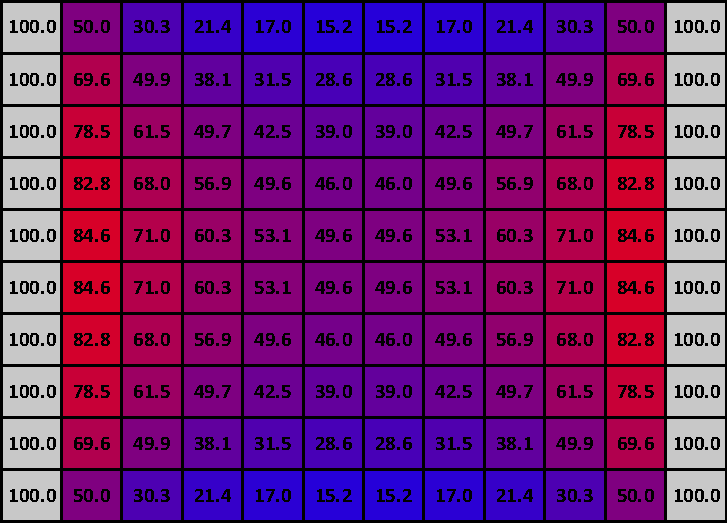
\includegraphics[width=0.6\textwidth]{papers/parallelisierung/images/simulation_10x10_0.135.pdf}
	\caption{Temperaturverteilung für \(10\times 10\)-Gitter, \(\lambda = 0.135\), nach Konvergenz.}
	\label{parallelisierung:fig:simulation_10x10_0.135}
\end{figure}

\paragraph{Fall 2: Instabile Simulation.}  
Erhöhen wir die Auflösung auf \(15\times 15\) Messpunkte (\(\Delta l = 0.006\,\mathrm{m}\)), bei gleichem \(\Delta t = 1\,\mathrm{s}\), daraus folgt
\[
\lambda =
\alpha \cdot \frac{\Delta t}{(\Delta l)^2}
=
1.355\cdot 10^{-5} \cdot \frac{1}{0.006^2}
\approx 0.376 > \frac14.
\]
Diese Parameter verletzen die aus \eqref{parallelisierung:eq:stabForExp} hervorgehende Stabilitätsbedingung. Somit ist nun mit einer Simulation zu rechnen, die nicht wie zuvor sauber konvergiert, sondern mit dem Fortschreiten der Zeit immer instabiler wird.

\begin{figure}[htbp]
	\centering
	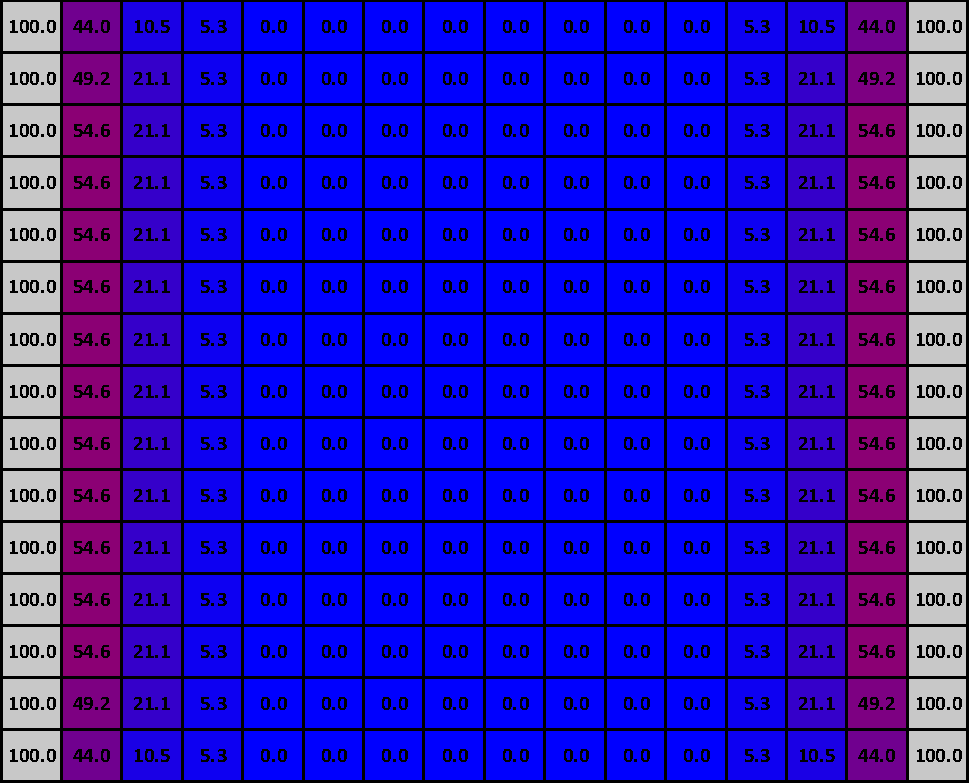
\includegraphics[width=0.8\textwidth]{papers/parallelisierung/images/simulation_15x15_0.376_3it.pdf}
	\caption{\(15\times 15\)-Gitter, \(\lambda = 0.376\), nach 3 Iterationen.}
	\label{parallelisierung:fig:simulation_15x15_0.376_3it}
\end{figure}

\begin{figure}[htbp]
	\centering
	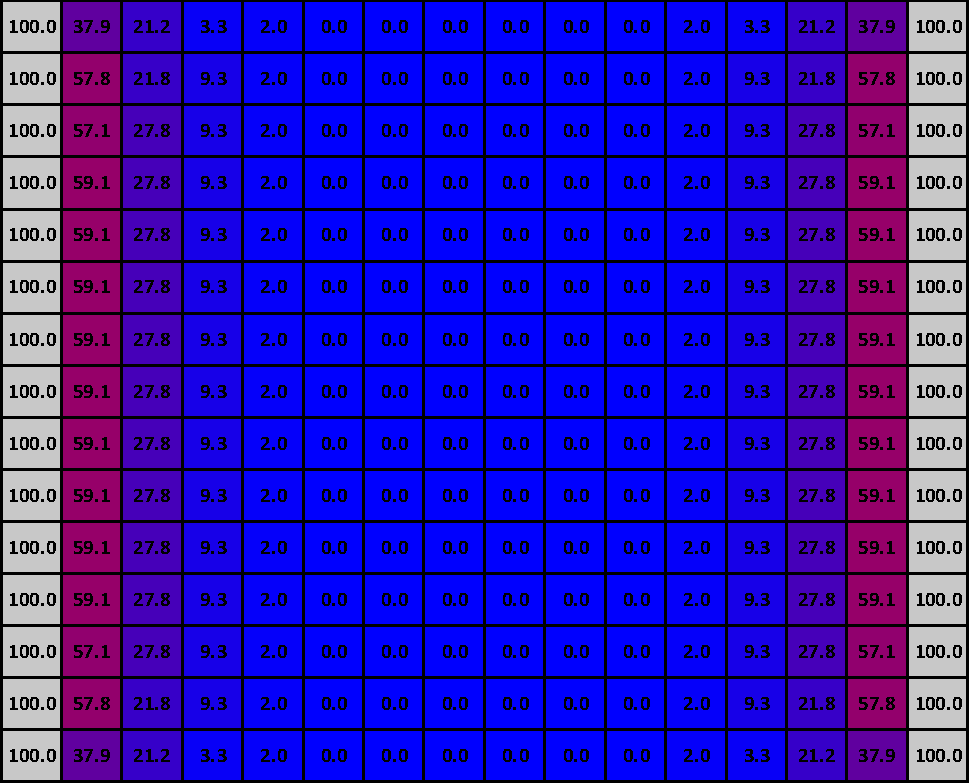
\includegraphics[width=0.8\textwidth]{papers/parallelisierung/images/simulation_15x15_0.376_4it.pdf}
	\caption{\(15\times 15\)-Gitter, \(\lambda = 0.376\), nach 4 Iterationen: erste Instabilitätsartefakte.}
	\label{parallelisierung:fig:simulation_15x15_0.376_4it}
\end{figure}

Zunächst scheint die Simulation noch plausibel (Abbildung~\ref{parallelisierung:fig:simulation_15x15_0.376_3it}), doch bereits nach wenigen weiteren Iterationen erscheinen die ersten auffälligen Werte (orange Zahlen in Abbildung~\ref{parallelisierung:fig:simulation_15x15_0.376_4it}). Anhand der physikalischen Intuition sowie den Ergebnissen der stabilen Simulation ist bekannt, dass das Temperaturgefälle von jeder Zelle in der oberen bzw. unteren Hälfte der Metallplatte bei jedem weiteren Schritt nach oben respektive unten entlang der orangen Pfeile streng monoton fallend sein muss. Das heisst, es kann nicht plötzlich wieder heisser werden, obwohl wir näher an den (kühlen) Rand gehen. Daraus lässt sich schliessen, dass die orange markierten Werte unphysikalisch und somit erste Instabilitäts-Artefakte sind.


Die Ursache lässt sich gut durch Umformung der expliziten Update-Formel 
\begin{equation}
	T_{i,j}^{n+1}
	=
	(1-4\lambda)T_{i,j}^n +
	\lambda \left(
	T_{i+1,j}^n + T_{i-1,j}^n + T_{i,j+1}^n + T_{i,j-1}^n
	\right)
\end{equation}
zeigen.
Für \(\lambda > \tfrac14\) wird der Koeffizient \((1-4\lambda)\) negativ, was wiederum bedeutet, dass das Zentrum negativ gewichtet wird.  
Dies führt dazu, dass Unterschiede zwischen benachbarten Zellen nicht geglättet, sondern verstärkt werden: es entstehen Über- und Unterschwinger, die sich mit jeder Iteration vergrössern.

\begin{figure}[htbp]
	\centering
	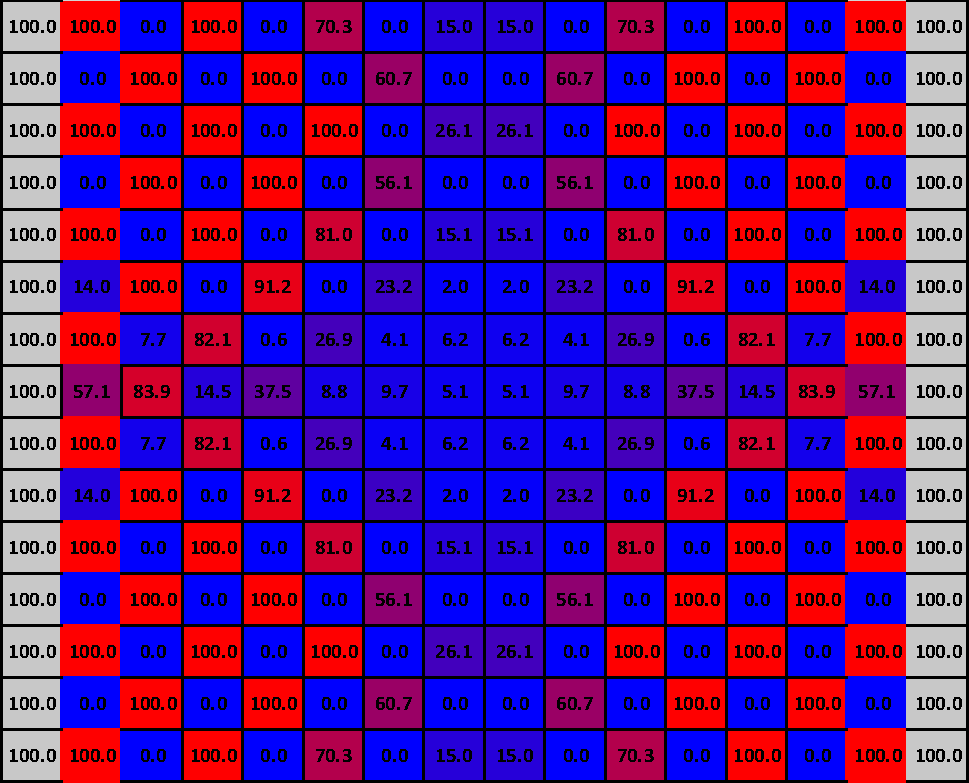
\includegraphics[width=0.8\textwidth]{papers/parallelisierung/images/simulation_15x15_0.376_15it.pdf}
	\caption{\(15\times 15\)-Gitter, \(\lambda = 0.376\), nach 15 Iterationen: klare Instabilitätsartefakte.}
	\label{parallelisierung:fig:simulation_15x15_0.376_15it}
\end{figure}

Lediglich zehn Iterationen später zeigt sich das Verhalten gemäss Abbildung~\ref{parallelisierung:fig:simulation_15x15_0.376_15it}, hier ist die Instabilität der Simulation aufgrund der Verletzung der 2D Stabilitätsbedingung mit \(\lambda = 0.376 > \frac{1}{4}\) deutlich sichtbar.

\paragraph{Fall 3: Wiederherstellung der Stabilität}  
Durch Verringerung von \(\Delta t\) auf \(0.5\,\mathrm{s}\) ergibt sich
\[
\lambda =
\alpha \cdot \frac{\Delta t}{(\Delta l)^2}
=
1.355\cdot 10^{-5} \cdot \frac{0.5}{0.006^2}
\approx 0.188 < \frac14.
\]
wodurch die Simulation wieder stabil wird. Die Konvergenz wird nach 315 Iterationen erreicht (Abbildung~\ref{parallelisierung:fig:simulation_15x15_0.188_konv}).

\begin{figure}[htbp]
	\centering
	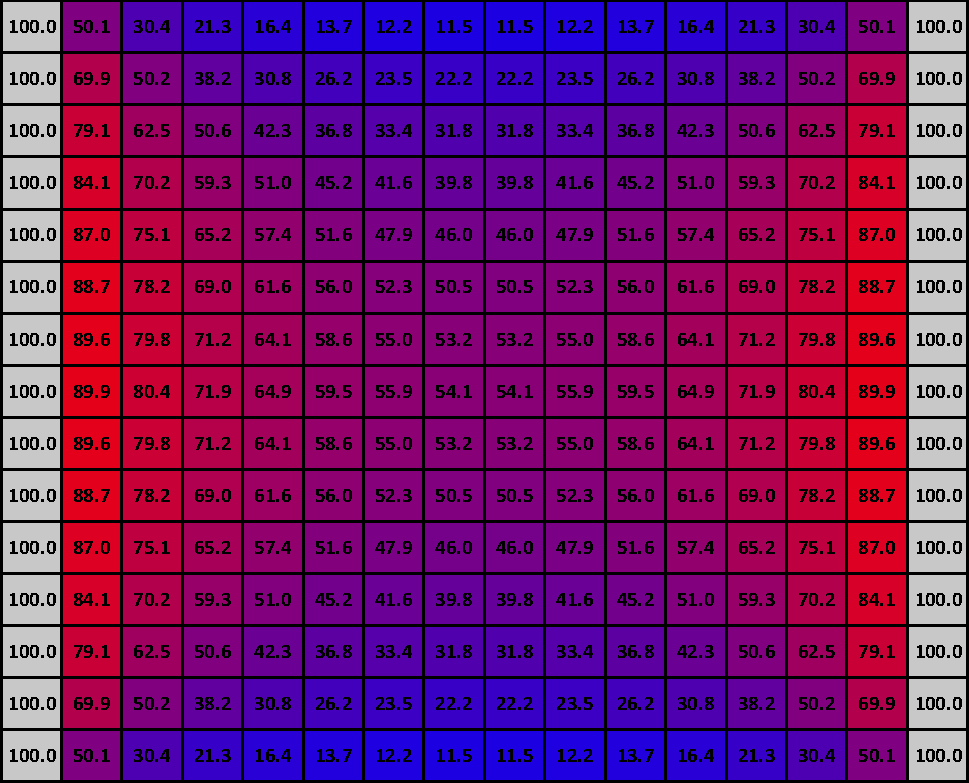
\includegraphics[width=0.8\textwidth]{papers/parallelisierung/images/simulation_15x15_0.188_konv.pdf}
	\caption{\(15\times 15\)-Gitter, \(\lambda = 0.188\), stabil nach Konvergenz.}
	\label{parallelisierung:fig:simulation_15x15_0.188_konv}
\end{figure}

